% todo-loop architecture: the context and memory model.
% Build with: latexmk -pdf context.tex   (or make -C docs/architecture)
\documentclass[11pt,a4paper]{article}

\usepackage[margin=1in]{geometry}
\usepackage{booktabs}
\usepackage{longtable}
\usepackage{listings}
\usepackage{xcolor}
\usepackage{microtype}
\usepackage{parskip}
\usepackage{enumitem}
\usepackage{caption}
\usepackage{tikz}
\usetikzlibrary{arrows.meta,positioning,fit,backgrounds}
\usepackage[hidelinks]{hyperref}

\definecolor{codebg}{gray}{0.96}
\definecolor{rule}{gray}{0.45}

\lstset{
  basicstyle=\ttfamily\footnotesize,
  backgroundcolor=\color{codebg},
  frame=single,
  rulecolor=\color{rule},
  breaklines=true,
  columns=fullflexible,
  keepspaces=true,
  showstringspaces=false,
  xleftmargin=0pt,
  framexleftmargin=3pt,
  framexrightmargin=3pt,
  aboveskip=\medskipamount,
  belowskip=\medskipamount,
}

\newcommand{\file}[1]{\texttt{#1}}
\newcommand{\key}[1]{\texttt{#1}}

\title{\textbf{todo-loop: the context and memory model}}
\author{Architecture notes}
\date{21 September 2026}

\begin{document}
\maketitle

\begin{abstract}
\noindent
todo-loop runs an unattended build as a sequence of single-task sessions, each
verified by a different model than the one that did the work. Its central
engineering problem is not planning and not verification --- it is context: a
27B worker with a 56{,}320-token window has to make progress on a project far
larger than that window, across dozens of sessions, on a 16\,GiB card it does
not have to itself.

This document describes where context lives, when it is deliberately destroyed
or compressed, and what occupies VRAM at each step. Numbers are measured on the
machine this was written on unless marked as derived. The headline result is
counterintuitive and worth stating up front: \emph{context management in this
system does not save any VRAM at all.} The KV cache is allocated in full when
the model loads and never changes size. Every byte of context discipline buys
prefill time and answer quality, not memory.
\end{abstract}

\tableofcontents
\clearpage

\section{The shape of the system}

\subsection{Two processes, two models}

A run is one long-lived driver process and a sequence of short-lived session
processes.

\begin{description}[leftmargin=1.5em,style=nextline]
  \item[The driver] \file{src/cli.ts}, invoked as \texttt{todo run}. A Node
  process that survives the whole run --- 7\,h\,38\,m in run~13. It owns the
  queue, decides which task is next, spawns a worker, applies the verdict,
  commits or reverts, and keeps count. It holds no model and uses no GPU.
  \item[The session] One \texttt{pi} process per iteration, spawned by
  \file{runPi} with \texttt{-p --approve} and, when \key{[project].packages} is
  set, \texttt{--no-extensions} plus one \texttt{-e} per package. It talks to
  the worker model, runs tools, and exits. Everything it learned dies with it.
  \item[The verifier] Not a session and not an agent. A single chat completion
  (\file{src/verify.ts}), given a system prompt and one user message, returning
  one JSON verdict. It has no tools, no history, and no memory of the previous
  task.
\end{description}

The asymmetry matters. The worker is an agent with a long, expensive, mutable
context. The verifier is a pure function from evidence to a boolean. Almost
everything in this document is about the first; \S\ref{sec:evidence} is the
only part about the second, and it is short because there is almost nothing
there by design.

\subsection{One task per session is the primary context mechanism}

The strongest context control in todo-loop is not a hook or a budget. It is the
decision that each task gets its own operating-system process, and that the
process exits when the task ends.

Nothing is carried forward implicitly. There is no rolling conversation, no
accumulated history, no summary of the last twelve tasks. Iteration $n{+}1$
starts with an empty context window and is handed, explicitly, only what
\S\ref{sec:channels} lists. A long run therefore has no context growth curve at
all --- it has 31 independent sawteeth, each starting at zero.

This is why the loop can run for eight hours on a window that holds perhaps
forty minutes of agent work. It never tries to hold the run in the window; it
holds one task, and writes down what the next one needs.

\section{Anatomy of one iteration}

\begin{figure}[ht]
\centering
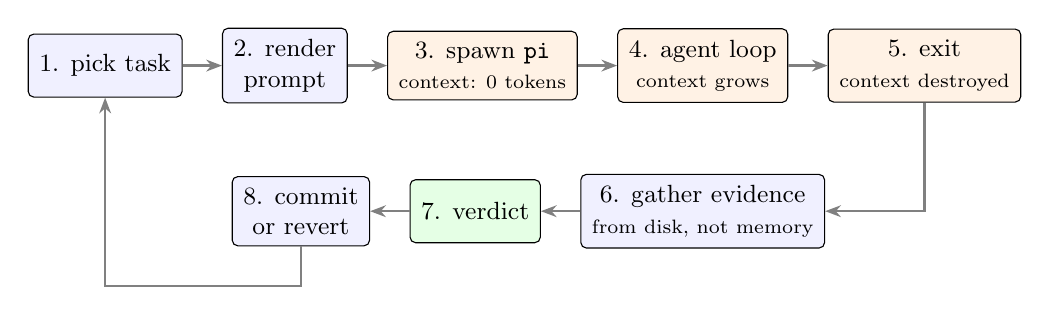
\begin{tikzpicture}[
  node distance=5mm,
  box/.style={draw, rounded corners=2pt, align=center, font=\small, inner sep=4pt, minimum height=8mm},
  drv/.style={box, fill=blue!6},
  ses/.style={box, fill=orange!10},
  ver/.style={box, fill=green!10},
  ->/.default=,
  arr/.style={-{Stealth[length=2mm]}, thick, draw=gray}
]
\node[drv] (pick)  {1. pick task};
\node[drv, right=of pick] (prompt) {2. render\\prompt};
\node[ses, right=of prompt] (spawn) {3. spawn \texttt{pi}\\\scriptsize context: 0 tokens};
\node[ses, right=of spawn] (work) {4. agent loop\\\scriptsize context grows};
\node[ses, right=of work] (exit) {5. exit\\\scriptsize context destroyed};

\node[drv, below=9mm of work] (gather) {6. gather evidence\\\scriptsize from disk, not memory};
\node[ver, left=of gather] (verify) {7. verdict};
\node[drv, left=of verify] (apply) {8. commit\\or revert};

\foreach \a/\b in {pick/prompt, prompt/spawn, spawn/work, work/exit}
  \draw[arr] (\a) -- (\b);
\draw[arr] (exit.south) |- (gather.east);
\draw[arr] (gather) -- (verify);
\draw[arr] (verify) -- (apply);
\draw[arr] (apply.south) -- ++(0,-0.5) -| (pick.south);
\end{tikzpicture}
\caption{One iteration. The only arrow that crosses the session boundary
carries files on disk, never model state.}
\label{fig:iteration}
\end{figure}

Steps 1--2 and 6--8 run in the driver. Steps 3--5 are the session. The break
between step~5 and step~6 is absolute: by the time evidence is gathered, the
worker no longer exists, and the evidence is read from the filesystem and from
git. This is why a worker cannot talk its way past verification --- the channel
through which it could is not connected.

\section{What crosses a session boundary}
\label{sec:channels}

Five channels, and no others.

\begin{longtable}{@{}p{0.26\textwidth}p{0.30\textwidth}p{0.36\textwidth}@{}}
\toprule
\textbf{Channel} & \textbf{Where} & \textbf{What it carries} \\
\midrule
\endhead
The queue & \file{todo.toml} & Task tree, statuses, and the \key{detail} text
that is the next worker's entire briefing. \\
\addlinespace
The memory file & \file{NOTES.md} (\key{plan.memory\_file}) & Durable findings
in the worker's own words. Read by every session, appended by any. \\
\addlinespace
The repository & git & The work itself. Also the verifier's evidence, via
\texttt{diff}. \\
\addlinespace
The sidecar & \file{*.todoloop-state.toml} & Attempts, timings, rejections.
Loop bookkeeping, never shown to a model except as \key{last\_failure}. \\
\addlinespace
The evidence file & \file{\$TMPDIR/todo-loop-evidence-*.md} & Output of tools
named in \key{verify.evidence\_tools}, captured as they ran. Truncated at the
start of every session. \\
\bottomrule
\end{longtable}

Only the first three reach a worker. The sidecar and the evidence file both
flow one way, into the driver and the verifier.

The memory file is the interesting one, because it is the only channel a worker
writes freely and a later worker reads in full. It is therefore the only place
where a wrong belief can propagate across sessions --- and run~13 shows both
faces of that. \file{NOTES.md} correctly recorded that \texttt{TonalIconButton}
does not exist in Material3 1.3, saving every later session the discovery. It
also recorded ``\textbf{THE decision}'' about rotated sliders, which compiled
and did not work, and every later session inherited it without question.

\subsection{The memory file has its own size discipline}

\file{src/notes.ts} meters the memory file as a \emph{share of the worker's
window}, not as a fixed byte count, because a fixed threshold eventually stops
meaning ``tidy this'' and starts meaning ``delete true facts until the number
is satisfied''.

\begin{lstlisting}
share = bytes / CHARS_PER_TOKEN / windowTokens     // CHARS_PER_TOKEN = 4
if (share <= plan.memory_share) -> none            // default 0.15
\end{lstlisting}

At the defaults that is $0.15 \times 56{,}320 \times 4 = 33{,}792$ bytes before
maintenance is queued. Run~13's \file{NOTES.md} reached 15{,}725 bytes, about
47\% of the way there.

When the tripwire does fire, the loop queues a compaction act and then judges it
\emph{by outcome} rather than by asking a model whether the file is tidy. A
compaction that sheds less than \texttt{MIN\_SHRINK} (10\%) has \emph{proven the
file compact}, and the file graduates to an index-plus-topic-files structure
instead of being compacted again. This is the same idiom the planner uses: a
planning round that adds nothing proves the branch done.

\section{In-session context management}

Inside a session, three pi hooks in \file{extension/index.ts} shape the window.
They fire at different times and do different jobs, and it is worth keeping them
apart.

\subsection{The entry cap: \texttt{tool\_result}}

Fires on every tool result, before anything enters the window. Pi's own cap is
50\,KB or 2000 lines, which is far too generous for a 27B. The extension
re-caps output from \texttt{BULKY\_TOOLS} at
\key{context.tool\_output\_max\_bytes} (default 2048), spills the full text to a
temp file, and appends a pointer to it.

Head or tail is chosen per tool: \texttt{TAIL\_TRUNCATED\_TOOLS} keep the end,
because for a build log the verdict is at the bottom. Everything else keeps the
head.

Two other things ride on this hook. \file{spendLook} meters a planning round's
inspection calls against \key{plan.look\_budget} (default 6) and, when spent,
injects a message that does not merely forbid the next call but names the exit:
an unanswered question becomes a research act. And \file{recordEvidence} appends
results from \key{verify.evidence\_tools} to the evidence file --- placed
before the hook's early returns, so a small result from an unspent budget still
reaches the verifier.

\subsection{The prune: the \texttt{context} hook}

Fires before each model call with the whole message list, and may rewrite it.

\begin{lstlisting}
if (usage.tokens < window * context.prune_at_fraction) return;   // 0.6
// walk back from the end; keep context.keep_full_turns assistant turns (3)
// everything before that cutoff:
//   assistant  -> trimThinking(message, context.thinking_keep_bytes)   // 600
//   toolResult -> if size >= context.stub_min_bytes (2000), replace with
//                 "[<tool> result elided - N bytes. Re-run the tool if
//                  you need it again.]"
\end{lstlisting}

Two design choices here are load-bearing.

\textbf{It is batched, not continuous.} llama.cpp and Ollama reuse the KV cache
only across a matching \emph{prefix}. Rewriting the middle of the history
invalidates everything after the edit and forces a recompute. Trimming a little
every turn would therefore mean a near-full prefill every turn. One large edit
at a threshold pays that cost once.

\textbf{Thinking is trimmed, not dropped.} Reasoning reaches the model only
when the provider replays it, which for the local worker means
\key{requiresThinkingAsText} in \file{\textasciitilde/.pi/agent/models.json}.
Before that flag, thinking was discarded every turn and the worker paid for it:
run~10 read the same file seven times and re-ran a grep eight minutes apart,
because conclusions it had already reached were never in front of it. Worse than
the re-reading, a worker with no trace of its own reasoning \emph{confabulates}
one --- asked to repeat a number it had chosen a turn earlier, it stated a
different number confidently rather than admitting the gap.

Replaying thinking in full brings back the opposite failure, where reasoning
accumulates until compaction fires and summarises thinking into yet more
context. A fixed tail is the middle: past \key{keep\_full\_turns} the retained
amount stops growing, so neither failure has room to develop. The tail rather
than the head, because a reasoning block spends most of itself getting somewhere
and states its conclusion at the end.

The effect is measurable on the wire. With \key{requiresThinkingAsText} on, each
turn's input grows by roughly the previous turn's entire output --- a ratio near
1.0; without it, about 0.56. Run~11 turn~3 emitted 4{,}948 output tokens and
turn~4's input rose by 4{,}986.

\textbf{\key{thinking\_keep\_bytes} has never fired in a live run.} It acts only
past \key{prune\_at\_fraction}, and no session has yet reached 60\% of 56{,}320
tokens $= 33{,}792$. The mechanism is tested but unexercised.

\subsection{The fallback: \texttt{session\_before\_compact}}

If a session does reach the point where pi compacts, the extension replaces the
default prose summary with fields:

\begin{lstlisting}
# Task state carried across compaction
task:          <id> [<kind>]: <title>
detail:        <the task's detail text>
attempt:       <n> of <max_attempts>
files_touched: <changed files>        (or added_this_round for a plan)
last_failure:  <reason>
Finish by calling todo_complete. Re-read any file you need; the
exploration that got you here is gone.
\end{lstlisting}

Fields rather than prose, because a prose summary loses exactly the details a
weak model needs in order to resume.

Compaction is also treated as \emph{evidence}. The hook sets
\file{compactedThisTask}, and at verification time that flags the leaf as having
overrun its budget --- the loudest available signal that the task was not atomic.
Depending on \key{atomic.on\_overflow} it is recorded or the task is promoted to
a plan.

\subsection{The pinned task}

One block is deliberately placed where none of the above can reach it.
\file{renderPinnedTask} puts the task id, ancestry, detail, and most recent
failure into the \emph{system} prompt. The comment in \file{src/prompt.ts} is
the whole rationale: \emph{the worker can lose its exploration; it must never
lose the task.}

\section{The verifier's context}
\label{sec:evidence}

The verifier gets one assembled string from \file{formatEvidence} and nothing
else --- no tools, no repository access, no conversation.

\begin{lstlisting}
## Task            id, title, detail
## Files changed   names only
## Diff            collectDiff(...), capped at verify.max_diff_bytes
## Command: <build_command>   exit code + output, capped at maxBytes/3
## Command: <test_command>    exit code + output, capped at maxBytes/3
## Tool evidence recorded during the session   capped at maxBytes/3
## Question        "Does the evidence above show that the task was done?"
\end{lstlisting}

Its system prompt is explicit that it is \emph{not} given the implementer's
account of what it did, and it judges the evidence only. That is the point of
the whole arrangement: the worker's narration is the one input a verifier must
never receive, because a model that has just spent thirty minutes on a task is
the worst available judge of whether the task is done.

\subsection{Two budgets, because the diff is not a log}

Until run~13 there was one knob, \key{verify.max\_evidence\_bytes} (12{,}000),
and \file{gatherEvidence} split it:

\begin{lstlisting}
const perPart = Math.max(1000, Math.floor(options.maxBytes / 3));   // 4000
\end{lstlisting}

So the diff --- the only artifact the verdict is actually about --- was capped
at \textbf{4000 bytes}, the same as each command's output. Run~13 showed the
cost. A research act whose entire work product \emph{was} its notes append had
its tail cut off, and the verifier, whose rules say to fail a diff that is
``obviously incomplete'', failed it. Twice, with the same words, because
\file{revertTo} restores the same tree and the retry reproduces the cut exactly.
The third attempt would have blocked the task on a defect the harness
introduced.

The diff now has its own budget, \key{verify.max\_diff\_bytes}, defaulting to
48{,}000 --- twelve times what it used to get. Command output keeps the thirds,
because a log compresses well: the tail carries the verdict and the rest is
noise. It remains a cap rather than unlimited, because a self-hosted verifier
has a window too and a runaway generated file should not be able to fill it.

Truncation markers now name their own author and their own size:

\begin{lstlisting}
[... truncated by todo-loop: showing the first 4000 of 21536 bytes;
 17536 bytes (81%) were dropped to fit the evidence budget, not
 omitted by the implementer ...]
\end{lstlisting}

and the verifier's rules gained a line saying that such a marker is the harness
trimming, not the implementer stopping early, and is never by itself grounds to
fail.

\section{VRAM: what is resident at each step}
\label{sec:vram}

\subsection{The measurement}

Taken from \texttt{nvidia-smi} and the Ollama API on the machine this run
executed on, with run~13's worker model resident.

\begin{longtable}{@{}lr@{}}
\toprule
\textbf{Quantity} & \textbf{Value} \\
\midrule
\endhead
GPU & NVIDIA RTX 2000 Ada Generation \\
Total VRAM & 16{,}380 MiB \\
\midrule
\texttt{llama-server} (the worker) & 13{,}530 MiB \\
\texttt{whisper-server} (unrelated, resident) & 1{,}916 MiB \\
\textbf{Total in use} & \textbf{15{,}527 MiB} \\
\textbf{Free} & \textbf{853 MiB} \\
\midrule
Model & \texttt{qwen3.8-27b:default} \\
Parameters & 27.3\,B \\
Quantisation & IQ3\_XXS (GGUF) \\
Weights on disk & 11{,}316 MiB \\
Reported \texttt{size\_vram} & 12{,}308 MiB \\
Configured \texttt{context\_length} & 56{,}320 tokens \\
\texttt{expires\_at} & year 2319 (i.e.\ \texttt{keep\_alive} never) \\
\bottomrule
\end{longtable}

Two derived figures, marked as derived because they are differences of reported
numbers rather than direct measurements:

\begin{itemize}[leftmargin=1.5em]
  \item \textbf{KV cache and graph $\approx$ 992 MiB}, from
  $12{,}308 - 11{,}316$. Over a 56{,}320-token window that is roughly
  18\,KiB per token.
  \item \textbf{CUDA context and compute buffers $\approx$ 1{,}222 MiB}, from
  $13{,}530 - 12{,}308$ --- the part \texttt{nvidia-smi} sees that Ollama's
  \texttt{size\_vram} does not report.
\end{itemize}

\subsection{The counterintuitive part: pruning frees nothing}

llama.cpp allocates the KV cache for the full \texttt{n\_ctx} when the model
loads. It does not grow as the conversation grows and it does not shrink when
the \texttt{context} hook elides half the history.

Therefore, at \emph{every} step of \emph{every} iteration --- driver picking a
task, session at turn one, session at turn forty, verifier running, driver
committing --- the GPU holds the same $\sim$13.5\,GiB. The occupancy is flat.

What context management actually buys is:

\begin{enumerate}[leftmargin=1.5em]
  \item \textbf{Prefill time.} Tokens in the window are tokens that must be
  attended over. At 10--12 tok/s generation on this box, prefill over a large
  prefix is a real fraction of a session.
  \item \textbf{Answer quality.} A 27B at IQ3\_XXS degrades with a window full
  of stale tool output long before it runs out of window.
  \item \textbf{Headroom against compaction}, which is expensive and lossy and
  is itself treated as an atomicity failure.
\end{enumerate}

It does \emph{not} buy memory. Any statement of the form ``pruning keeps us from
running out of VRAM'' is false on this architecture. The only lever that changes
VRAM is \texttt{n\_ctx} at load time --- which is why the Ollama tag list carries
\texttt{:16k}, \texttt{:21k}, \texttt{:28k}, \texttt{:42k}, \texttt{:47k},
\texttt{:52k}, \texttt{:55k}, \texttt{:56k} and \texttt{:73k} variants of the
same weights. Choosing a tag is choosing a KV allocation.

\subsection{Why the verifier is hosted}

With 853 MiB free, there is no room for a second model. A self-hosted verifier
would have to evict the worker, and Ollama would then reload 11\,GiB of weights
from disk to bring the worker back for the next task --- twice per iteration,
every iteration, for a verdict that is a few hundred tokens of output.

Run~13's 31 iterations would have paid that swap 62 times. This is the concrete
reason \key{models.verifier} points at a hosted endpoint, and it is a capacity
decision rather than a quality one.

It also explains the \key{[ollama]} config block's existence. A local verifier
invoked through a session goes via pi's model registry and picks up
\file{models.json}; \texttt{todo complete} from the command line has no session
and no registry, so it talks to the server directly. The block exists so those
two paths cannot disagree about the same model. Its defaults are Qwen's own
thinking-mode recommendation, and the trap worth naming is that
\texttt{temperature 0} --- which looks correct for a judge --- is what makes
Qwen's thinking mode loop.

\subsection{The container boundary}

Android builds do not run on the host. \file{/data/android/build.sh} executes
Gradle inside a per-project container, and the emulator is a separate container
again. Neither touches the GPU. The relevance to this document is timing rather
than memory: \texttt{docker run} on a warm image costs 11--28\,s on this box
because container creation is effectively serialised in \texttt{dockerd}, while
\texttt{docker exec} into a live container costs about 80\,ms. The persistent
builder exists for that reason and took repeat builds from 25\,s to 2\,s.

A slow build is a context problem in disguise: every second the worker waits is
a second of a 30-minute budget, and run~13 lost ten sessions to that budget.

\section{Budget reference}

\begin{longtable}{@{}llp{0.42\textwidth}@{}}
\toprule
\textbf{Key} & \textbf{Default} & \textbf{What it bounds} \\
\midrule
\endhead
\key{context.prune\_at\_fraction} & 0.6 & Window fraction before the prune
fires. Never reached in any run so far. \\
\key{context.keep\_full\_turns} & 3 & Assistant turns kept verbatim at the tail. \\
\key{context.stub\_min\_bytes} & 2000 & Smallest tool result worth eliding. \\
\key{context.tool\_output\_max\_bytes} & 2048 & Cap on bulky tool output
\emph{entering} the window at all. \\
\key{context.thinking\_keep\_bytes} & 600 & Tail of each old thinking block
kept when the prune fires. \\
\midrule
\key{verify.max\_diff\_bytes} & 48000 & The diff's own budget. New in run~13. \\
\key{verify.max\_evidence\_bytes} & 12000 & Split three ways across command
output and tool evidence. \\
\key{verify.max\_attempts} & 3 & Attempts before a task blocks. \\
\midrule
\key{plan.memory\_share} & 0.15 & Window share \file{NOTES.md} may cost. \\
\key{plan.memory\_window\_tokens} & 56320 & The window that share is taken of. \\
\key{plan.look\_budget} & 6 & Inspection calls in a planning round. \\
\key{plan.max\_children} & 5 & Items one planning round may add. \\
\midrule
\key{atomic.max\_files} & 5 & Files a leaf may touch before it counts as
overflowed. Known wrong for a scaffold, which touches about twelve. \\
\key{loop.worker\_timeout\_ms} & --- & 1{,}800{,}000 in the eq2 config. \\
\key{loop.plan\_timeout\_ms} & --- & 600{,}000 in the eq2 config. \\
\bottomrule
\end{longtable}

\section{What the model does not reach}

It is worth listing the deliberate exclusions, because several were bugs before
they were features.

\begin{itemize}[leftmargin=1.5em]
  \item \textbf{Sibling task details.} Only titles, and only for boundary-setting
  (\file{siblingTitles}). A sibling's full record would pull far more into the
  window than it returns.
  \item \textbf{The queue file itself.} Workers get a rendered prompt, not
  \file{todo.toml}. A fifty-task tree is not a briefing.
  \item \textbf{\key{project.setup\_command} and \key{teardown\_command}.} Run by
  the driver around the run. The model never sees them; it finds the emulator
  already booted.
  \item \textbf{The sidecar.} Attempts and timings are the loop's bookkeeping.
  Only \key{last\_failure} is surfaced, and only into the pinned block.
  \item \textbf{The previous session's anything.} No transcript, no summary, no
  rolling state.
\end{itemize}

\section{Known gaps}

\begin{enumerate}[leftmargin=1.5em]
  \item \textbf{\key{thinking\_keep\_bytes} is untested in production}
  (\S\ref{sec:vram} notwithstanding, no session has crossed
  \key{prune\_at\_fraction}).
  \item \textbf{Nothing measures prefill cost.} The batched-prune design is
  justified by how llama.cpp reuses a KV prefix, but the saving has never been
  instrumented on this box.
  \item \textbf{No cross-module evidence.} The verifier sees one diff at a time.
  Run~13 shipped a unit mismatch --- millihertz and millibels read as hertz and
  decibels --- that survived 28 consecutive passing verifications because each
  side of the seam was correct on its own terms and no gate looks at both.
  \item \textbf{\key{atomic.max\_files} does not fit a scaffold.}
  \item \textbf{The memory file has no correctness gate.} Size is metered;
  truth is not. A confidently wrong note propagates to every later session.
\end{enumerate}

\end{document}
